\section{Change of assumptions}

\section{Architecture of your module}
The module \texttt{gossip} has been developed using the Golang programming language. It relies heavily on Go features like goroutines, Go channels, and multiple Go libraries. 

\subsection{The whole picture}

As the specification requires, the \texttt{gossip} module runs as two independent protocols: one API protocol and one P2P protocol. However, these two protocols share some data to fulfill the functionality of the module. 

\begin{figure}[h]
    \centering
    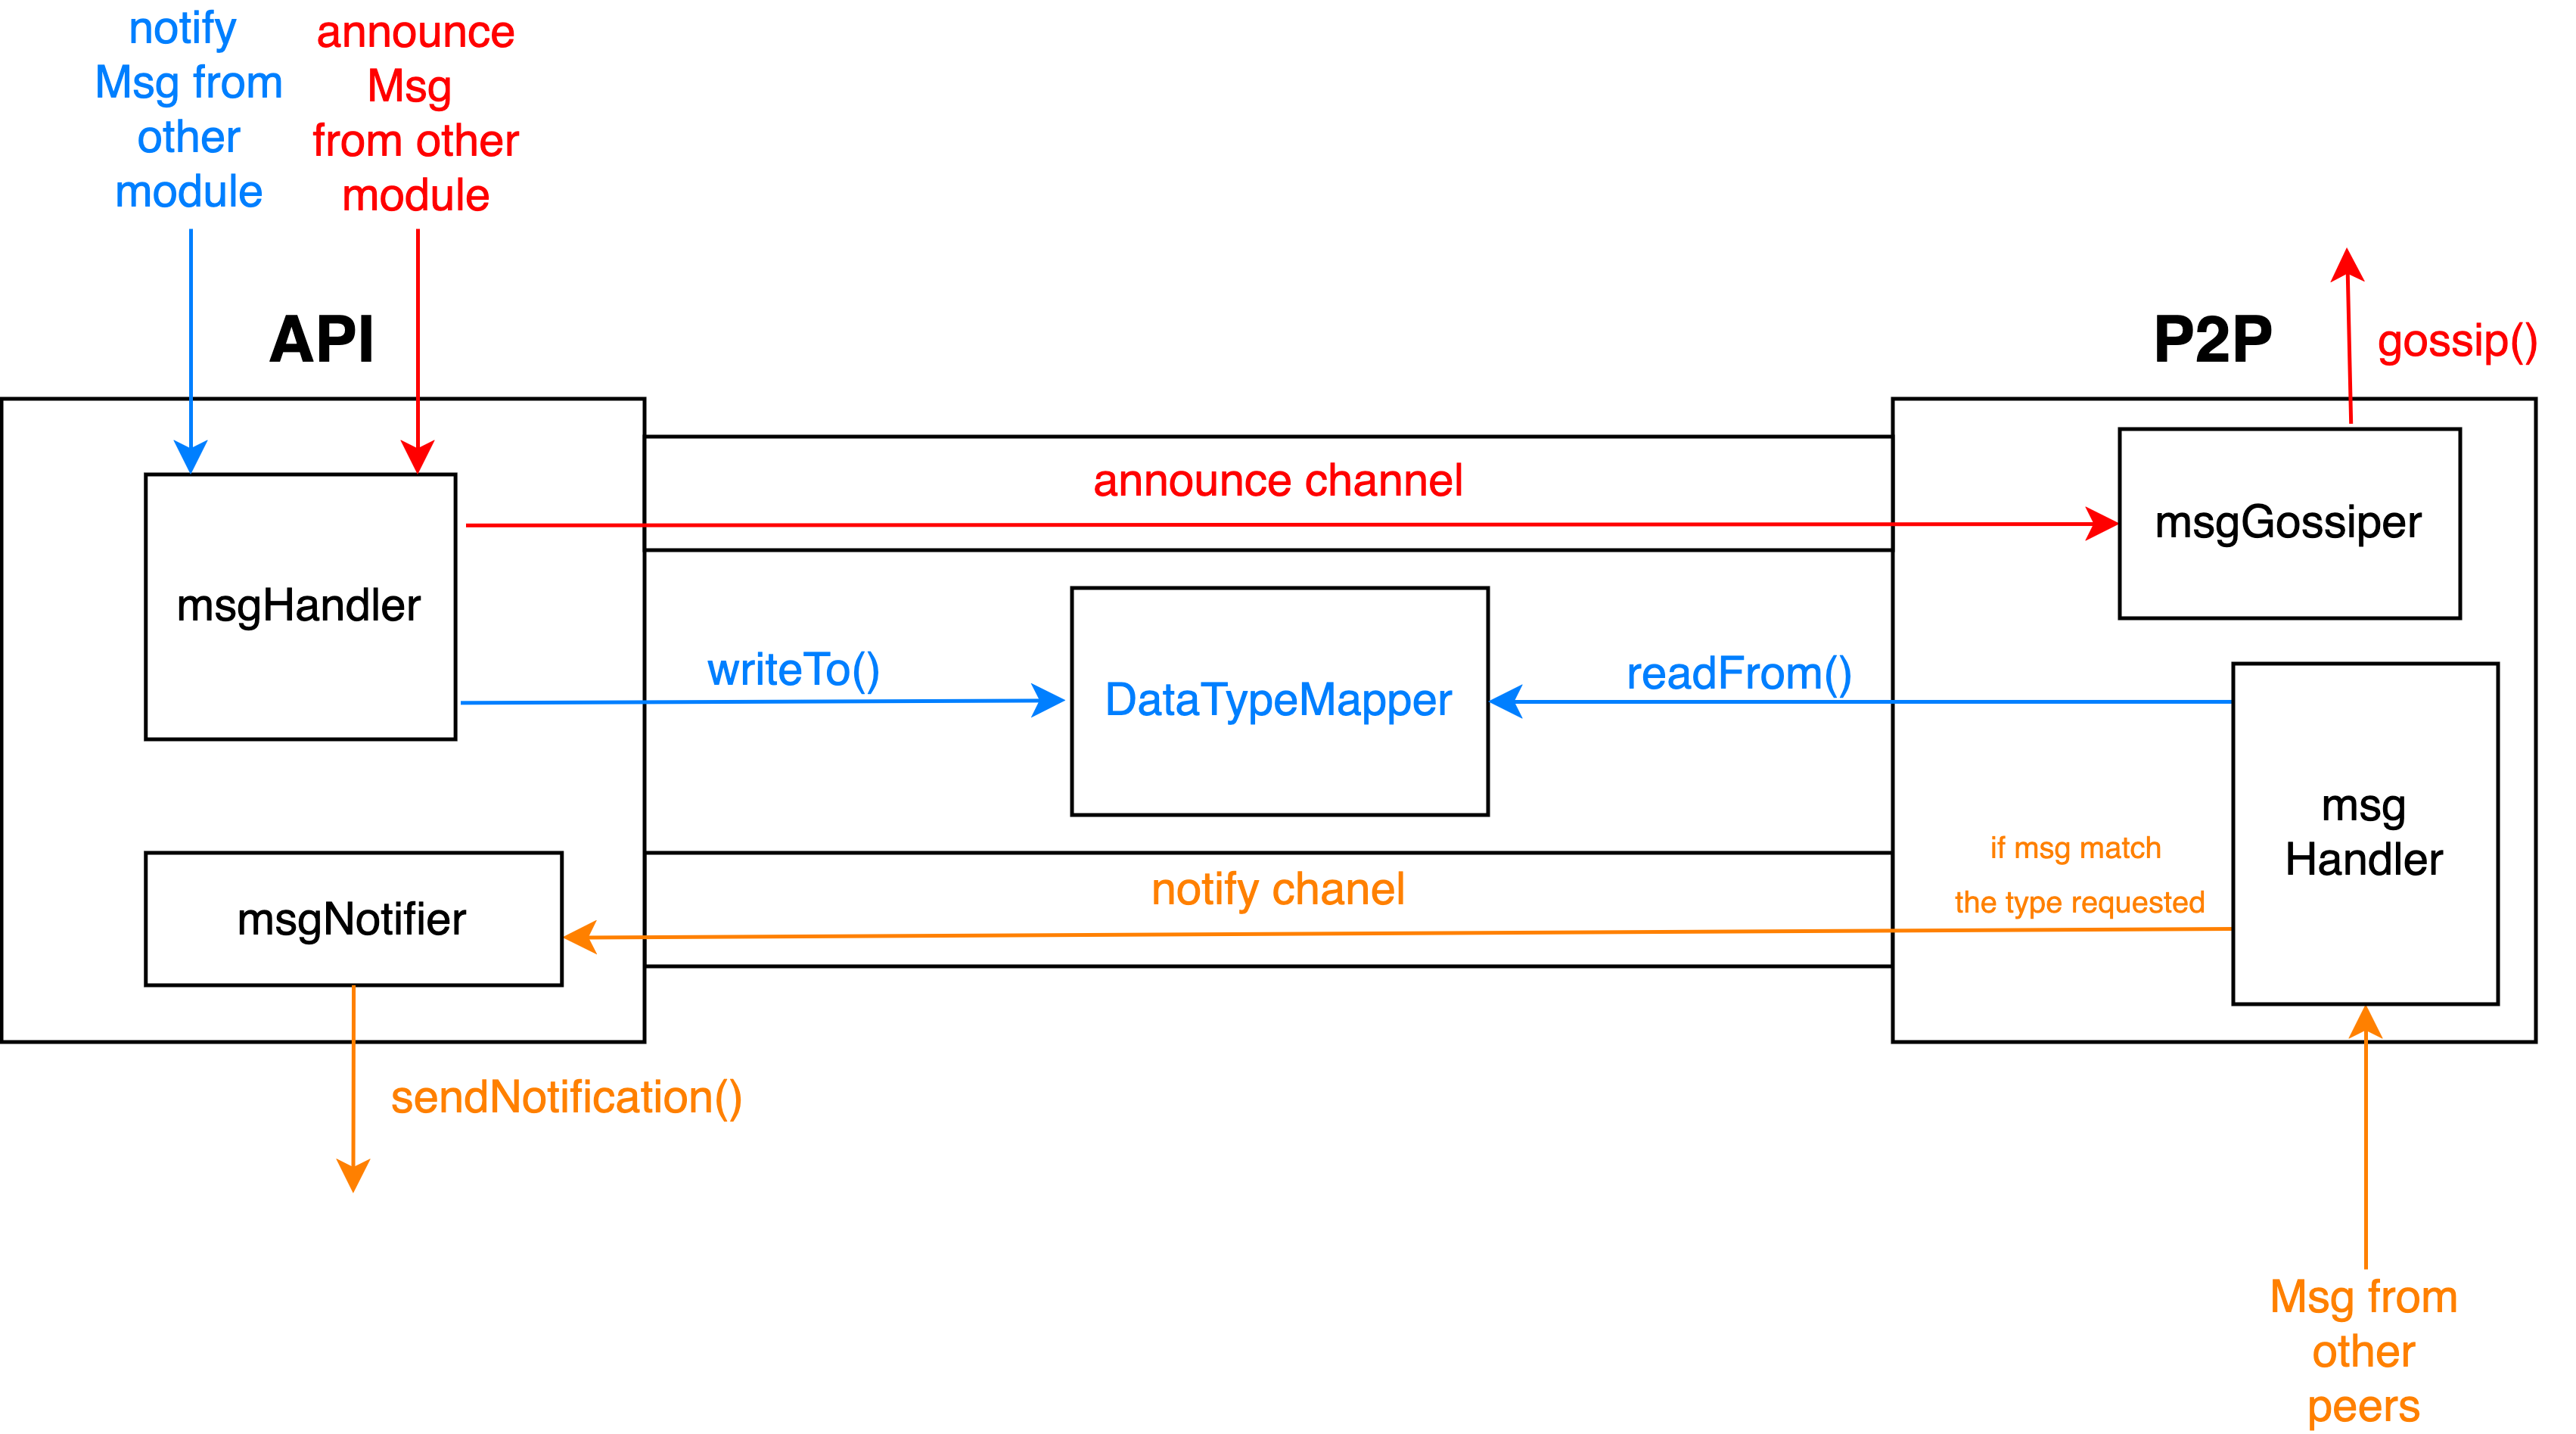
\includegraphics[width=0.8\textwidth]{pics/structure.png}
    \caption{Structure of the gossip module}
\end{figure}

\subsubsection{1. Announce messages Go channel}

To make the announce functionality work, we need an \textbf{announce Go channel}\footnote{Marked in red in Figure 1} shared between the two protocols. Whenever the API protocol receives an announce message from another module, it processes the message immediately and sends it to the P2P protocol through this channel. The P2P protocol has an announce message handler running on a goroutine that always listens to this channel. When it receives an announce request, it will gossip this message away. 

\begin{lstlisting}
announceMsgChan := make(chan enum.AnnounceMsg)
\end{lstlisting}

\subsubsection{2. Datatype mapper}

To make the notify functionality work, we need a \textbf{datatype mapper}\footnote{Marked in blue in Figure 1} shared between two protocols. Whenever API receives a notify message, it will write the message type that is valid into the mapper and hence should be propagated further. This datatype mapper will, of course, own a mutex that guarantees there is no race condition between the two protocols.

\begin{lstlisting}
type DatatypeMapper struct {
    mutex sync.RWMutex
    data  map[net.Addr]map[enum.Datatype]bool
}
\end{lstlisting}

\subsubsection{3. Notify messages Go channel}

Thanks to the datatype mapper, the P2P protocol can recognize which kind of message it should propagate. When it receives a new message, it will check if this message type was requested by any module by reading the datatype mapper. If that is the case, it sends this message through \textbf{notify message Go channel}\footnote{Marked in orange in Figure 1}. API protocol also has a running goroutine that constantly listens to this channel. It can get those messages from P2P and send corresponding notification messages to the module requesting them. 

\subsection{API}

The API is designed to facilitate a Gossip-based protocol in a distributed system, leveraging Go's robust features for concurrency and networking. At its core, the Server listens on a specified TCP address for incoming connections, using Go's net package to manage network communications. Once a connection is accepted, the Server hands it off to a Handler, which processes messages according to their type.

The Handler utilizes a custom logger for monitoring and error reporting, enhancing the system's reliability and debuggability. It reads incoming messages, verifies their size and type using the bytes and encoding/binary packages, and then routes them to the appropriate handler functions. These functions handle specific message types such as announcements or notifications, updating the datatypeMapper, or sending messages to the announceMsgChan channel as necessary.

This seamless interaction between the Server and Handler ensures the system can efficiently process and route messages, maintaining data integrity and system state across distributed nodes. The use of Go's concurrency primitives, like goroutines and channels, allows the API to handle multiple connections simultaneously, making it scalable and robust for real-time, distributed communication.


\subsection{P2P}

TODO: Trung

\section{Security Measures}

\section{Specification of the peer-to-peer protocol that will be implemented}

\section{Future Work}

\section{Workload distributed}

\section{Effort spent for the project}